\documentclass{exos}
\usepackage{main}

\begin{document}
\begin{exercize}
Exprimer les situations suivantes à l'aide d'une expression algébrique :
\begin{alphaquestions}
\item Quel est l'expression de l'aire du triangle rectangle $ABC$ suivant ?
\begin{center}
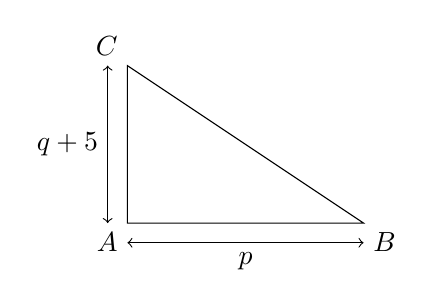
\begin{tikzpicture}
\coordinate (A) at (0,0);
\coordinate (B) at (3,0);
\coordinate (C) at (0,2);

\draw (A) -- (B) -- (C) -- cycle;
\draw (A) node[below left] {$A$};
\draw (B) node[below right] {$B$};
\draw (C) node[above left] {$C$};
\draw[<->] ([yshift=-0.25cm]A) -- ([yshift=-0.25cm]B) node[midway,below] {$p$};
\draw[<->] ([xshift=-0.25cm]A) -- ([xshift=-0.25cm]C) node[midway,left] {$q + 5$};
\end{tikzpicture}
\end{center}
\item Jérémy vient de terminer un repas au restaurant, et constate que le prix de son dessert vaut trois fois le prix de son entrée (qui coûte $c$ €), et son plat principal vaut le double de son dessert. Combien a-t-il payé en tout ?
\end{alphaquestions}
\end{exercize}
\vspace*{2cm}
\begin{exercize}
Exprimer les situations suivantes à l'aide d'une expression algébrique :
\begin{alphaquestions}
\item Quel est l'expression de l'aire du triangle rectangle $ABC$ suivant ?
\begin{center}
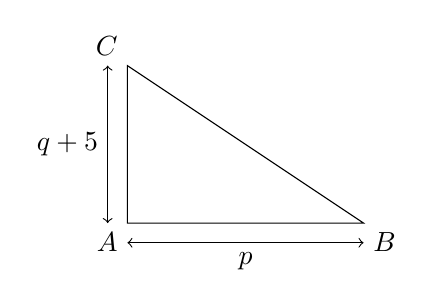
\begin{tikzpicture}
\coordinate (A) at (0,0);
\coordinate (B) at (3,0);
\coordinate (C) at (0,2);

\draw (A) -- (B) -- (C) -- cycle;
\draw (A) node[below left] {$A$};
\draw (B) node[below right] {$B$};
\draw (C) node[above left] {$C$};
\draw[<->] ([yshift=-0.25cm]A) -- ([yshift=-0.25cm]B) node[midway,below] {$p$};
\draw[<->] ([xshift=-0.25cm]A) -- ([xshift=-0.25cm]C) node[midway,left] {$q + 5$};
\end{tikzpicture}
\end{center}
\item Jérémy vient de terminer un repas au restaurant, et constate que le prix de son dessert vaut trois fois le prix de son entrée (qui coûte $c$ €), et son plat principal vaut le double de son dessert. Combien a-t-il payé en tout ?
\end{alphaquestions}
\end{exercize}
\end{document}